%-------------------------------------------------------------------------%
% ARCHIVO: img_tex/diagrama.tex
% Arreglado con desactivación local para babel (spanish)
%-------------------------------------------------------------------------%
\shorthandoff{>} % Apaga el conflicto del español justo antes de empezar

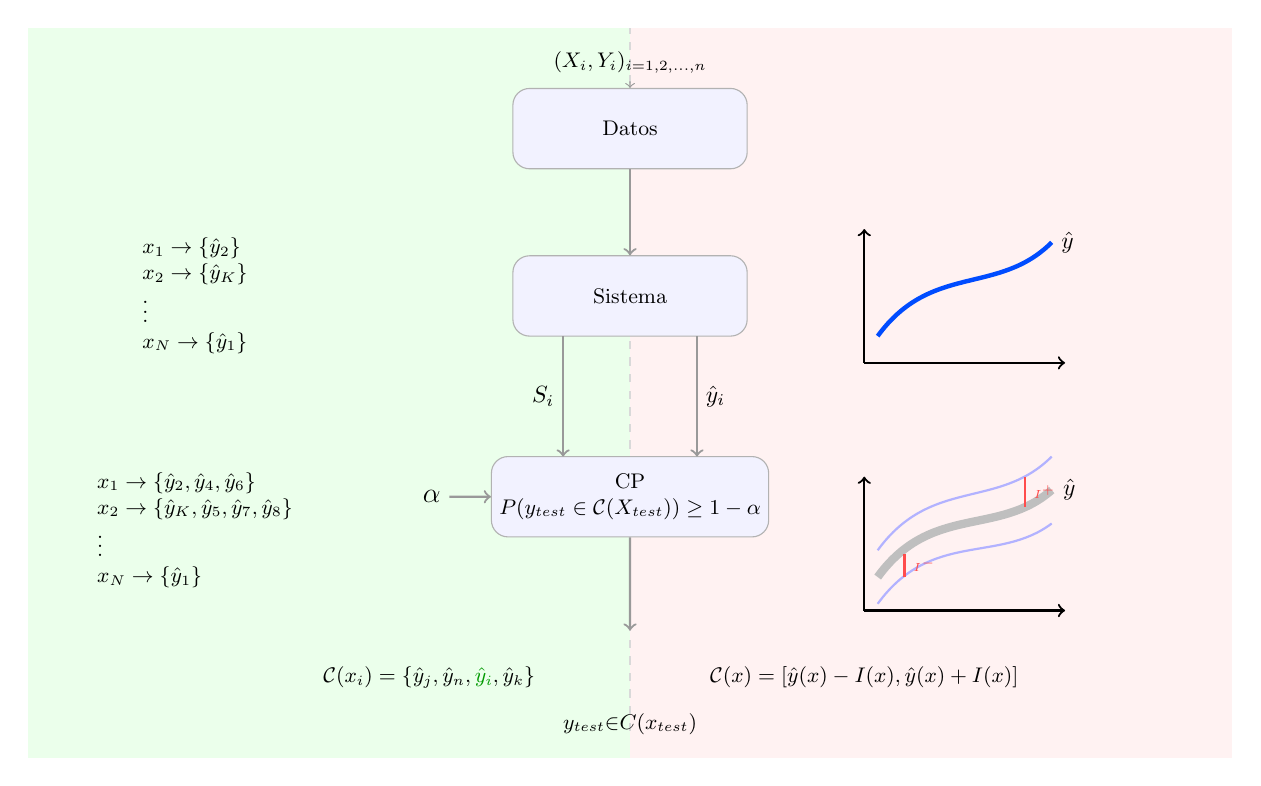
\begin{tikzpicture}[
    scale=0.85, every node/.style={transform shape},
    % Estilos de los bloques centrales
    bloque/.style={rectangle, draw=gray!60, fill=blue!5, rounded corners=6pt, minimum width=3.5cm, minimum height=1.2cm, align=center, font=\small},
    % Estilo para el texto de las ecuaciones
    textoEq/.style={align=left, font=\small}
]

% 1. FONDOS DE COLORES (Izquierda Verde, Derecha Rosa)
\fill[green!8] (-9, -5.4) rectangle (0, 5.5); % Subí un poquito el fondo (de 5 a 5.5) para que tape la nueva ecuación
\fill[red!5] (0, -5.4) rectangle (9, 5.5);
\draw[gray!30, dashed] (0, -5) -- (0, 5.5); 

% 2. BLOQUES CENTRALES Y FLECHAS
% Agregamos la ecuación arriba de Data en (0, 4.9)
\node[font=\small] (dataset) at (0, 4.99) {$(X_i, Y_i)_{i=1,2,\dots, n}$};

\node[bloque] (data) at (0, 4) {Datos};
\node[bloque] (sistema) at (0, 1.5) {Sistema};
\node[bloque] (cp) at (0, -1.5) {CP \\ $\mathbb{P}(y_{\text{test}} \in \mathcal{C}(X_{\text{test}})) \ge 1-\alpha$};

\node[textoEq] at (0, -4.9) {$y_{test} \mathcal \in {C}(x_{test}) $};

% Flecha delgada desde la nueva ecuación hacia el bloque Data
\draw[->, gray!80, thin] (dataset) -- (data);

\draw[->, gray!80, thick] (data) -- (sistema);
\draw[->, gray!80, thick] (-1, 0.9) -- node[left, black] {$S_i$} (-1, -0.9);
\draw[->, gray!80, thick] (1, 0.9) -- node[right, black] {$\hat{y}_i$} (1, -0.9);
\draw[->, gray!80, thick] (cp) -- (0, -3.5);

% Parámetro alpha apuntando a CP
\draw[->, gray!80, thick] (-2.7, -1.5) node[left, black, font=\large] {$\alpha$} -- (cp);

% 3. LADO IZQUIERDO (Clasificación - Verde)
\node[textoEq] at (-6.5, 1.5) {
    $x_1 \rightarrow \{\hat{y}_2\}$ \\
    $x_2 \rightarrow \{\hat{y}_K\}$ \\
    $\vdots$ \\
    $x_N \rightarrow \{\hat{y}_1\}$
};

\node[textoEq] at (-6.5, -2) {
    $x_1 \rightarrow \{\hat{y}_2, \hat{y}_4, \hat{y}_6\}$ \\
    $x_2 \rightarrow \{\hat{y}_K, \hat{y}_5, \hat{y}_7, \hat{y}_8\}$ \\
    $\vdots$ \\
    $x_N \rightarrow \{\hat{y}_1\}$
};

\node[textoEq] at (-3, -4.2) {$\mathcal{C}(x_{i}) = \{\hat{y}_j, \hat{y}_n, \textcolor{green!60!black}{\hat{y}_{i}}, \hat{y}_k\}$};


% 4. LADO DERECHO (Regresión - Rosa)

% Gráfico Superior (Predicción puntual)
\begin{scope}[shift={(3.5, 0.5)}]
    \draw[->, thick] (0,0) -- (3,0);
    \draw[->, thick] (0,0) -- (0,2);
    % Curva azul de predicción
    \draw[blue!70!cyan, ultra thick] (0.2, 0.4) .. controls (1, 1.5) and (2, 1) .. (2.8, 1.8) node[right, black] {$\hat{y}$};
\end{scope}

% Gráfico Inferior (Intervalos de confianza / bandas)
\begin{scope}[shift={(3.5, -3.2)}]
    \draw[->, thick] (0,0) -- (3,0);
    \draw[->, thick] (0,0) -- (0,2);
    
    % Banda superior (azul claro)
    \draw[blue!30, thick] (0.2, 0.9) .. controls (1, 2) and (2, 1.5) .. (2.8, 2.3);
    % Banda inferior (azul claro)
    \draw[blue!30, thick] (0.2, 0.1) .. controls (1, 1.2) and (2, 0.7) .. (2.8, 1.3);
    % Curva central (gris gruesa)
    \draw[gray!50, line width=3pt] (0.2, 0.5) .. controls (1, 1.6) and (2, 1.1) .. (2.8, 1.8) node[right, black] {$\hat{y}$};
    
    % Etiquetas de las bandas I+ e I-
    \draw[red!70, thick] (2.4, 1.55) -- node[right, font=\tiny] {$I^+$} (2.4, 2.0);
    \draw[red!70, thick] (0.6, 0.5) -- node[right, font=\tiny] {$I^-$} (0.6, 0.85);
\end{scope}

\node[textoEq] at (3.5, -4.2) {$\mathcal{C}(x) = [\hat{y}(x) - I(x), \hat{y}(x) + I(x)]$};

\end{tikzpicture}

\shorthandon{>} % Lo vuelve a encender para que el resto del texto de tu informe funcione bien